\chapter*{\textsc{Statement of Originality}}
\vspace{-0.5cm}

This is to certify that to the best of my knowledge, the content of this thesis is my own work and is based on research conducted during my PhD candidature at The University of Sydney, except where noted below:

\vspace{0.5cm}

In Chapter \ref{chap:red_giants}, the raw image-subtracted light curves were extracted by Isabel Colman \citep{colman_pixels_2020}. I produced the target list for selecting the stars Isabel extracted, and performed all of the corrections and analysis for these light curves.

\vspace{0.5cm}

Chapter~\ref{chap:fluffy} of this thesis is published as \cite{drury_large_2017}. 
It should be noted that the data used in this chapter are based on the same raw data as the thesis {\it `Photometry of the Kepler Superstamps: A method for obtaining a complete sample of open cluster stars'} submitted as part of my Graduate Diploma of Science. However, I re-extracted and reduced the data and obtained additional observations through collaborations, the analysis of which completely changed its variable classification. As such the analysis presented in this thesis is original. The multi-colour photometry was obtained by Aliz Derekas, L\'aszl\'o Szigeti, R\'obert Szak\'ats, Kriszti\'an S\'arneczky, and L\'aszl\'o Moln\'ar. The identification of chemically peculiar signatures was performed by Simon Murphy, and the model-based rotational modulation stability analysis was conducted by \'Ad\'am S\'odor.

\vspace{0.5cm}

This thesis has not been submitted for any degree or other purposes. I certify that the intellectual content of this thesis is the product of my own work and that all the assistance received in preparing this thesis and sources have been acknowledged.

\vspace{1cm}

\begin{figure}[!h]
\centering
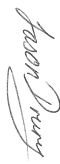
\includegraphics[width=0.1\textwidth,angle=90]{Chapter_Preface/signature.png}
\end{figure}
\begin{center}
Jason Andrew Drury
\end{center}
